\documentclass[tikz, border=3pt]{standalone}

\usepackage{tikz}
\usetikzlibrary{calc}

\begin{document}
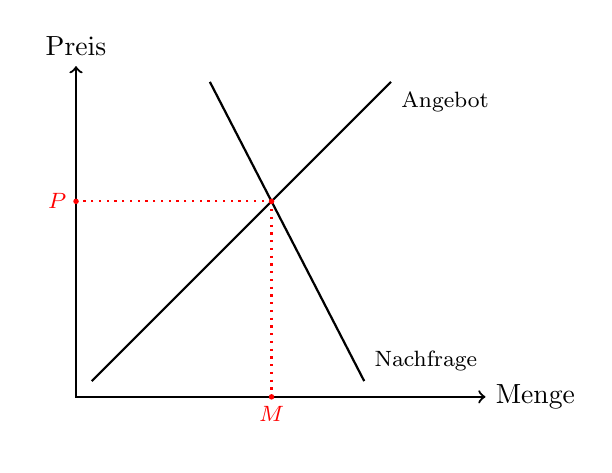
\begin{tikzpicture}
	
	\draw[thick] (.2,.2) coordinate (a1) -- (4,4) coordinate (a2) node[below right, text width=5em] {\footnotesize Angebot};
	\draw[thick] (1.7, 4) coordinate (b1) -- (3.66, .2) coordinate (b2) node[above right, text width=5em] {\footnotesize Nachfrage};
	
	\fill[red] (intersection cs: first line={(a1) -- (a2)}, second line={(b1) -- (b2)}) coordinate (i1) circle (1pt);
	
	
	
	
	\draw[thick, red, dotted] let \p1 = (i1) in (i1) -- (\x1,0) coordinate (e1);
	\draw[thick, red, dotted] let \p1 = (i1) in (i1) -- (0,\y1) coordinate (e3);
	

	\draw [<->, thick] (0,4.2) node (yaxis) [above] {Preis} |- (5.2,0) node (xaxis) [right] {Menge};
	
	
	\draw[->, thick, white] let \p1 = (e3), \p2 = (e3) in (-.6, \y1) -- (-.6, \y2);
	\draw[->, thick, white] let \p1 = (e1), \p2 = (e1) in (\x1,-.6) -- (\x2, -.6);
	
	
	
	\fill[red] (e1) circle (1pt)  node[below] {\footnotesize $M$};
	\fill[red] (e3) circle (1pt)  node[left] {\footnotesize $P$};
	
\end{tikzpicture}
\end{document} 